\documentclass{standalone}
\usepackage{pgfplots}
\pgfplotsset{soldot/.style={color=black,only marks,mark=*},
             holdot/.style={color=black,fill=white,only marks,mark=*},
             compat=1.12}
\begin{document}
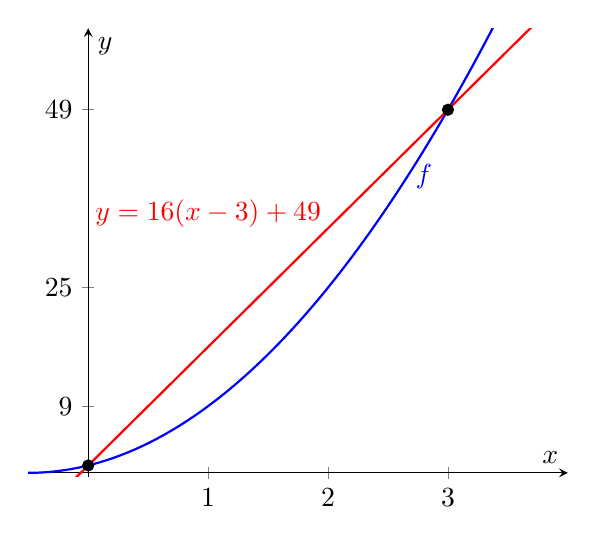
\begin{tikzpicture}
\begin{axis}[
 axis lines=middle,
 %ticklabel style={fill=blue!5!white},
 xmin=-.5,xmax=4,
 ymin=-.5,ymax=60,
 xtick={1,2,3},xticklabels={1,2,3},
 ytick={9,25,49},   yticklabels={9,25,49},       %<--
% minor tick = {-5,-3,...,5}, %<--
 xlabel=\(x\),ylabel=\(y\),
 samples=200]

\addplot[domain=-2:7,thick,blue] {4*x^2+4*x+1};
\addplot[domain=-2:7,thick,red] {16*(x-3)+49};
\addplot[soldot] coordinates{(3,49)(0,1)};

\draw [blue] (axis cs:2.8,40)  node [] {$f$};
\draw [red] (axis cs:1,35)  node [] {$y=16(x-3)+49$};


\end{axis}
\end{tikzpicture}
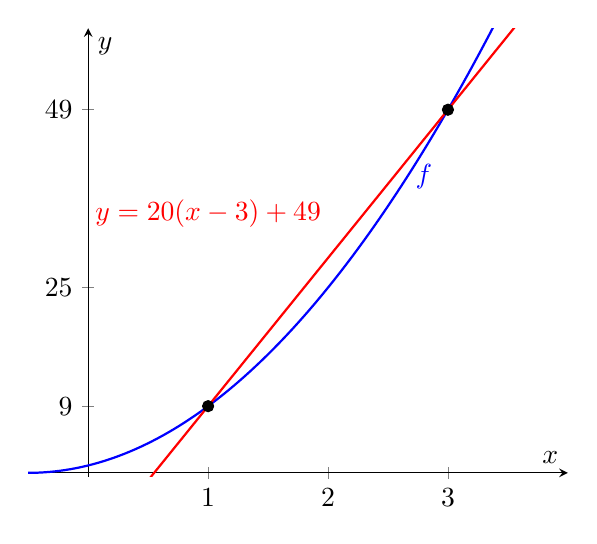
\begin{tikzpicture}
\begin{axis}[
 axis lines=middle,
 %ticklabel style={fill=blue!5!white},
 xmin=-.5,xmax=4,
 ymin=-.5,ymax=60,
 xtick={1,2,3},xticklabels={1,2,3},
 ytick={9,25,49},   yticklabels={9,25,49},       %<--
% minor tick = {-5,-3,...,5}, %<--
 xlabel=\(x\),ylabel=\(y\),
 samples=200]

\addplot[domain=-2:7,thick,blue] {4*x^2+4*x+1};
\addplot[domain=-2:7,thick,red] {20*(x-3)+49};
\addplot[soldot] coordinates{(3,49)(1,9)};

\draw [blue] (axis cs:2.8,40)  node [] {$f$};
\draw [red] (axis cs:1,35)  node [] {$y=20(x-3)+49$};


\end{axis}
\end{tikzpicture}
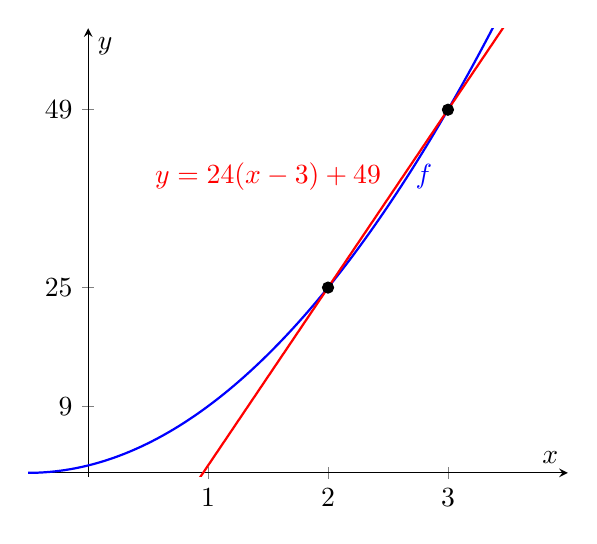
\begin{tikzpicture}
\begin{axis}[
 axis lines=middle,
 %ticklabel style={fill=blue!5!white},
 xmin=-.5,xmax=4,
 ymin=-.5,ymax=60,
 xtick={1,2,3},xticklabels={1,2,3},
 ytick={9,25,49},   yticklabels={9,25,49},       %<--
% minor tick = {-5,-3,...,5}, %<--
 xlabel=\(x\),ylabel=\(y\),
 samples=200]

\addplot[domain=-2:7,thick,blue] {4*x^2+4*x+1};
\addplot[domain=-2:7,thick,red] {24*(x-3)+49};
\addplot[soldot] coordinates{(3,49)(2,25)};

\draw [blue] (axis cs:2.8,40)  node [] {$f$};
\draw [red] (axis cs:1.5,40)  node [] {$y=24(x-3)+49$};


\end{axis}
\end{tikzpicture}
\end{document}